\documentclass[10pt,a4paper]{article}
\usepackage{nips15submit_e}
\usepackage{amsmath}
\usepackage{mathtools}
\usepackage{amsfonts}
\usepackage{amssymb}
\usepackage{graphicx}
\usepackage{float}
\usepackage{hyperref}
%\usepackage[
%backend=bibtex,
%sorting=unsrt
%]{biblatex}
%\addbibresource{projectsources.bib}
\usepackage{xcolor}
\usepackage{algorithmicx}
\usepackage{algpseudocode}
\usepackage{setspace}

\usepackage[paperwidth=8.5in,paperheight=11in,centering,hmargin=1in,vmargin=1in]{geometry}
\nipsfinalcopy

%\DeclarePairedDelimiter{\norm}{\lVert}{\rVert}
\usepackage{physics}
\newcommand{\prox}{\mathrm{prox}}
\newcommand{\R}{\mathbb{R}}
\newcommand{\C}{\mathbb{C}}
\newcommand{\Tau}{\mathcal{T}}
\newcommand{\AMz}{\underset{z}{arg\, min}}

\begin{document}
\title{Image Deblurring and Denoising \\with Various Fidelity Terms and Regularizers}
\author{
Kelsey Maass, ~Samuel Rudy, ~Kevin Mueller, ~and Riley Molloy\\
University of Washington\\
}

\maketitle

\begin{center}
\begin{minipage}{0.8\textwidth}
\begin{center}
\textbf{Abstract}
\end{center}
weeee worm weeee worm weeee worm weeee worm weeee worm weeee worm weeee worm weeee worm weeee worm weeee worm weeee worm weeee worm weeee worm weeee worm weeee worm weeee worm weeee worm weeee worm weeee worm weeee worm weeee worm weeee worm weeee worm weeee worm weeee worm weeee worm weeee worm weeee worm weeee worm weeee worm weeee worm weeee worm weeee worm weeee worm weeee worm weeee worm 
\end{minipage}
\end{center}

% Introduction
\section{Introduction}
Image denoising and deblurring problems can be modeled with the linear system
\begin{equation}
Ax + w = b,
\end{equation}
where $b$ is the observed image, $w$ is some unknown noise, and $x$ is the true image we would like to recover. For a blurred image we let $A$ represent the blurring process, and for noisy images we let $A$ be the identity matrix. For many inverse problem applications the least squares approximation, 
\begin{equation}
\hat{x}_{LS} = \arg\min_x \| Ax - b \|_F^2 ,
\end{equation}
gives a reasonable solution. Unfortunately, this approach doesn't provide any new information for the denoising problem, and for image deblurring problems $A$ is often ill-conditioned, so the solution is contaminated by round-off error and amplified noise. To illustrate this, we consider the pepper image below. If we blur the image and compute the naive solution $x = A^{-1}b$, the result is obscured by round-off error in the form of ringing artifacts. The result is even worse when we add noise.

\begin{figure}[H]
\centering
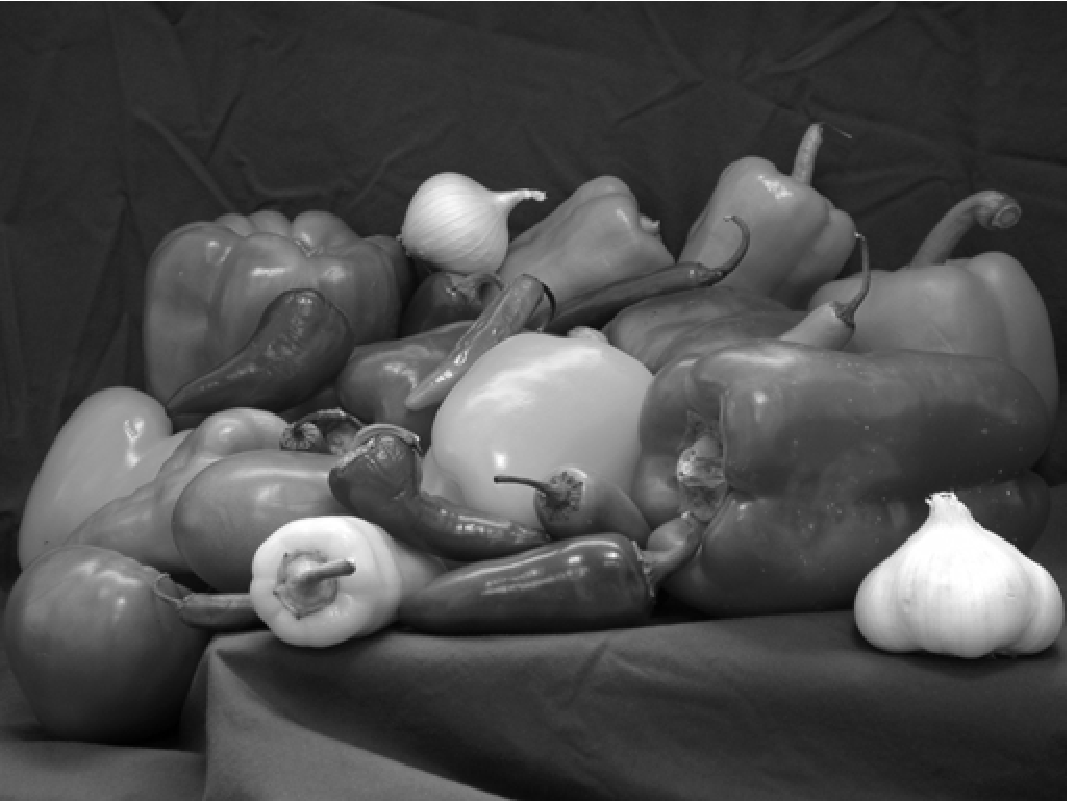
\includegraphics[width=2in]{../figures/fig1}
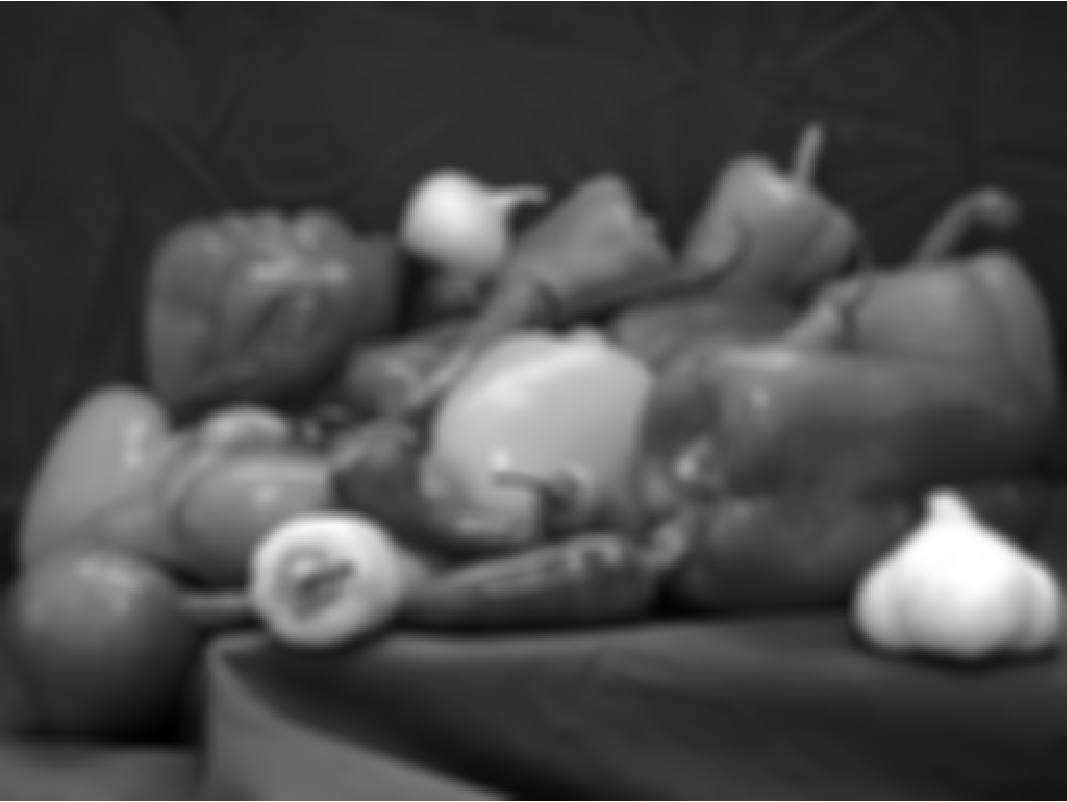
\includegraphics[width=2in]{../figures/fig2}
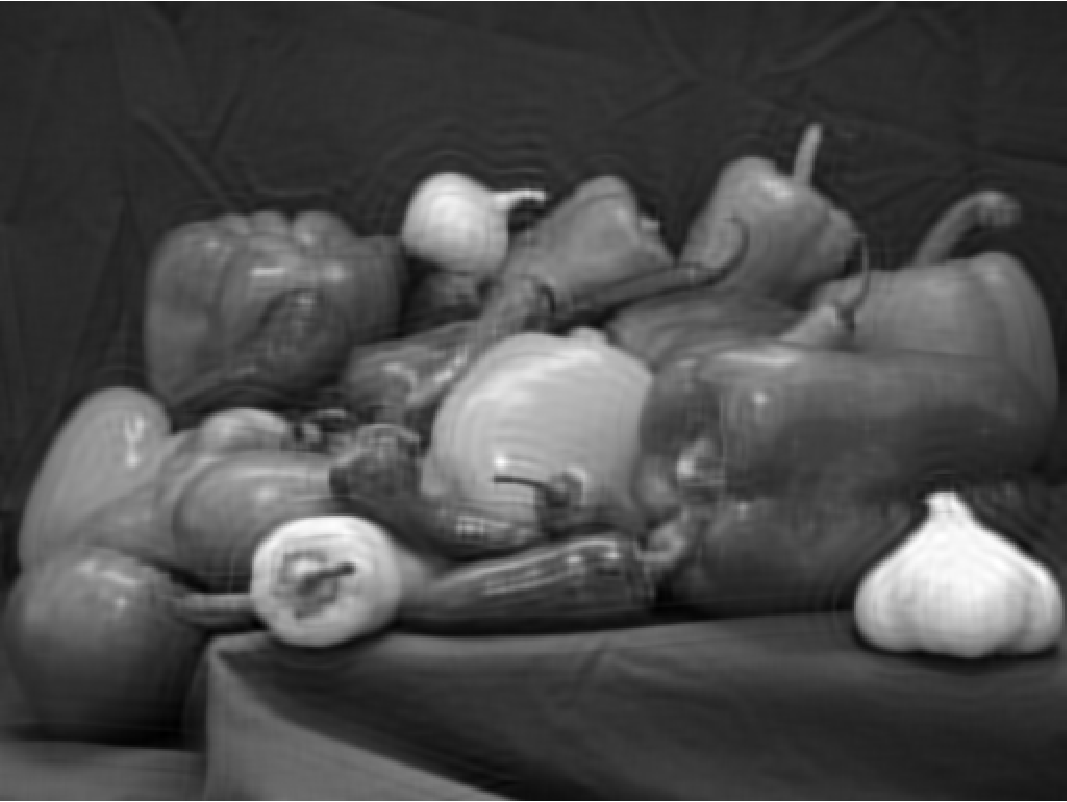
\includegraphics[width=2in]{../figures/fig3} \\[1ex]
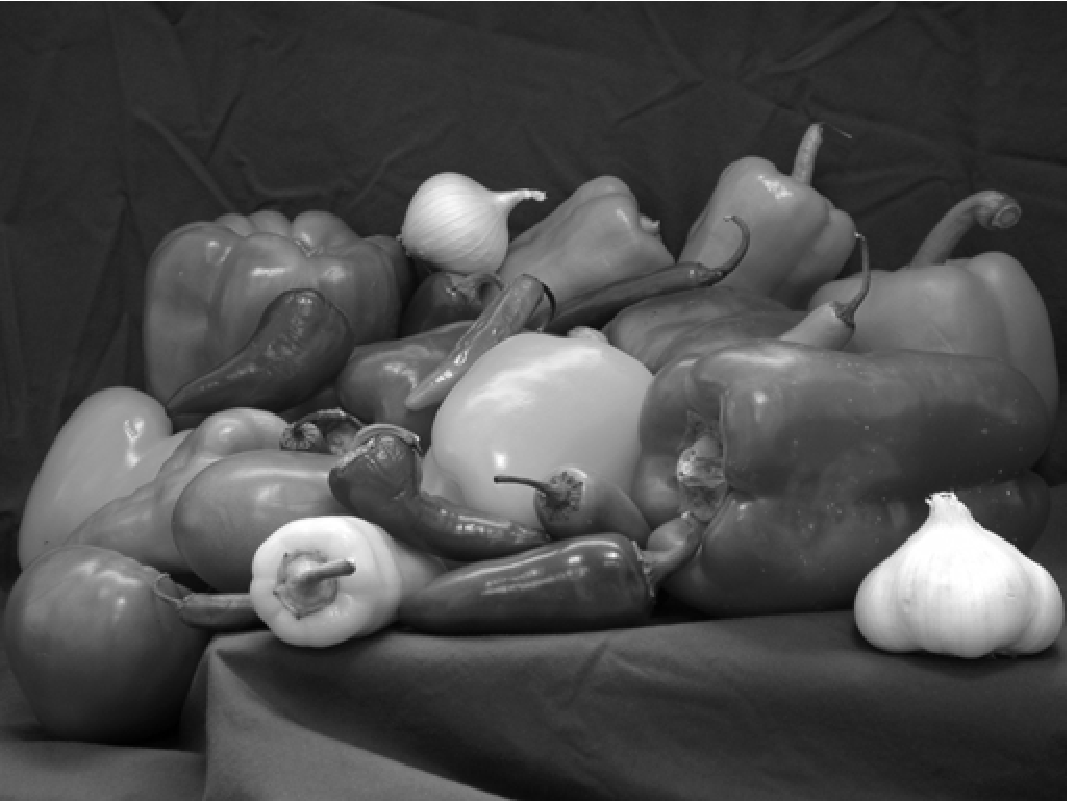
\includegraphics[width=2in]{../figures/fig1}
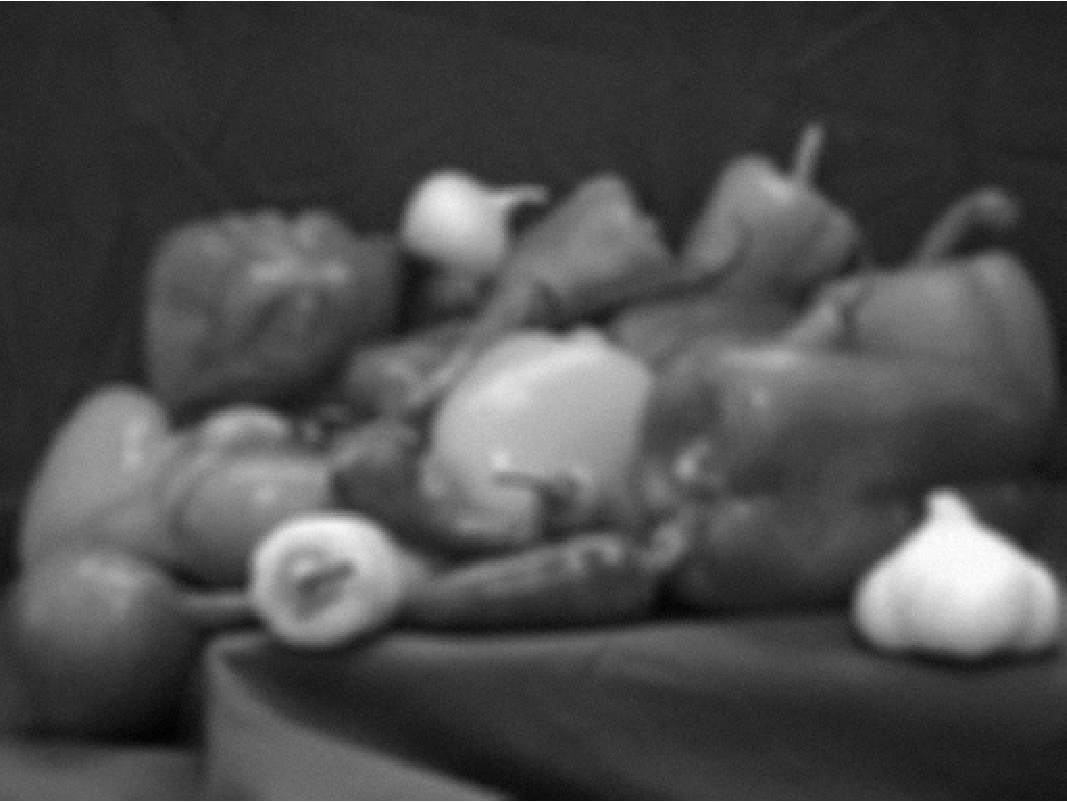
\includegraphics[width=2in]{../figures/fig4}
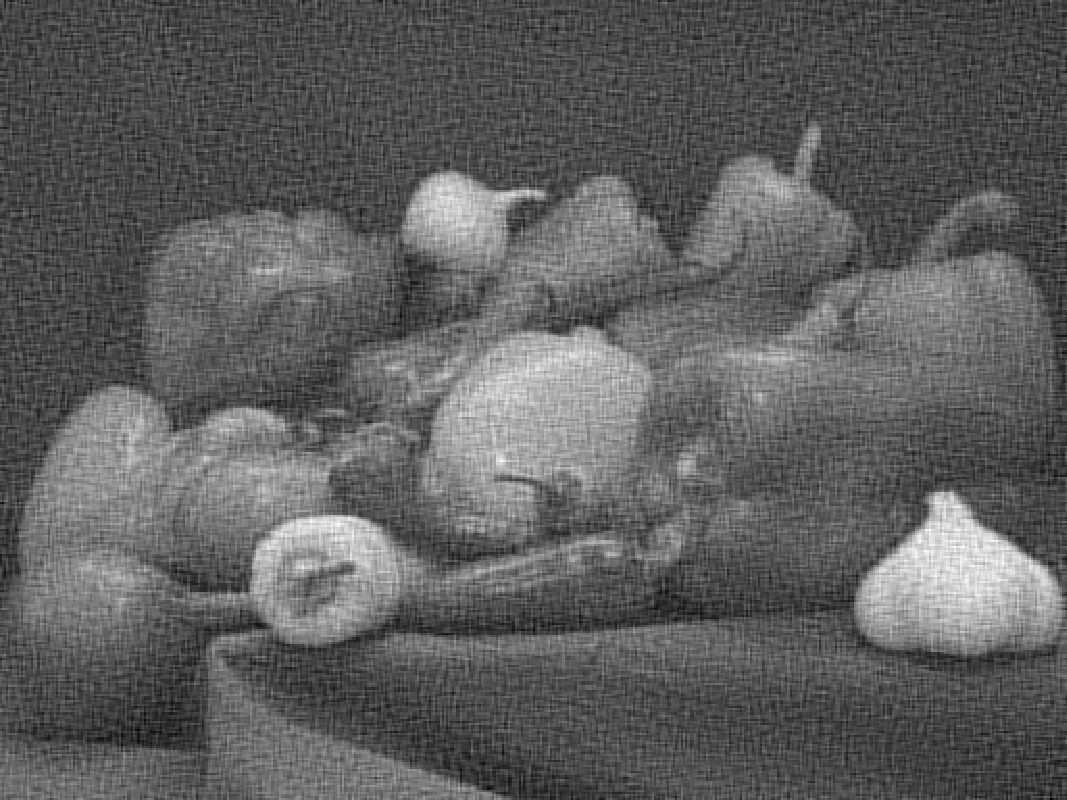
\includegraphics[width=2in]{../figures/fig5}
\caption{\small In the top row we observe the naive solution applied to a blurred image, including the true image $x$ (left), the blurred image $b$ (middle), and the recovered image $A^{-1}b$. On the bottom row, we see the effects of adding noise illustrated by the true image $x$ (left), the blurred and noisy image $b-w$ (middle), and the recovered image $A^{-1}(b-w)$.}
\end{figure}

In order to stabilize the solution, a variety of regularizers can be used which exploit features of the true image such as smoothness or sparsity in a wavelet domain. This results in the problem formulation
\begin{equation}
\hat{x} = \arg\min_{x} \| Ax - b \|_F^2 + \lambda R(x),
\end{equation}
where the parameter $\lambda > 0$ is chosen to balance the tradeoff between fidelity to the model and the assumed feature. In this paper we compare two choices for the regularization term: $\ell_1$ wavelet regularization with $R(x) = \| Wx \|_1$, and total variation regularization with $R(x) = TV(x)$, which are explored by Beck and Teboulle in \cite{TV} and \cite{FISTA} respectively.
%\begin{align}
%&\text{Total variation regularization:} &\hat{x}_{TV} = \arg\min_x \| Ax - b \|_F^2 + 2\lambda \| x \|_{TV} , \\
%&\text{and } \ell_1 \text{ regularization:} &\hat{x}_{\ell_1} = \arg\min_x \| Ax - b \|_F^2 + \lambda \| Wx \|_1  ,
%\end{align}



It is also known that the quadratic penalty is extremely sensitive to outliers. While this does not pose problems for images with Gaussian noise, which may result from atmospheric turbulence, it becomes an issues for images with noise from heavier tailed distributions, such as the Student's t-distribution, which could result from a dirty camera lens. Therefore we also consider different choices for the fidelity term which are more robust to outliers than the quadratic penalty, including the Huber norm
\begin{equation} \label{huber}
h_{\gamma}(x) = \min_y \frac{1}{2} \| x - y \|_F^2 + \gamma \| y \|_1,
\end{equation}
and the function
\begin{equation} \label{log_cosh}
g_{\gamma}(x) = \frac{1}{\gamma} \sum_i \log\left(\cosh\left(\gamma x_i\right)\right).
\end{equation}

We note that $g_{\gamma}(x)$ approaches the $\ell_1$ penalty uniformly as we increase $\gamma$, leading to linear penalization. The Huber penalty, on the other hand, approaches a linear penalty as we decrease $\gamma$, but with an increasingly smaller slope.

\begin{figure}[H]
\centering
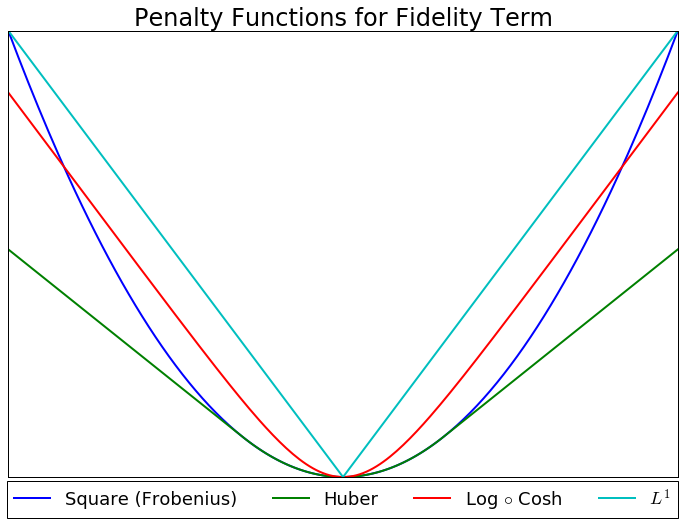
\includegraphics[width=0.8\textwidth]{../figures/penalty_functions.png} 
\caption{al;sdfj?}
\end{figure}

% Problem Formulation
\section{Problem Formulation}
The general approach to the image deblurring and denoising problem can now be stated as a minimization problem of the form \cite{DeblurBook}
\begin{equation} \label{general}
 \min_x f(Ax -b) + \lambda R(x),
\end{equation}
where $Ax$ is a discrete convolution of the true image with a blur kernel, the  \emph{fidelity term} $f(Ax-b)$ measures how well the recovered image complies with the linear model, and $R(x)$ is our chosen \emph{regularization}. The parameter $\lambda > 0$ is chosen to balance the tradeoff between fidelity to the model and noise sensitivity. Furthermore, if we assume that the pixels of our image satisfy $x_{i,j} \in [0,1]$, we can add an additional term to the objective function
\begin{equation} \label{loss}
 L_b(x) = f(Ax-b) + \lambda R(x) + \delta(x | [0,1] ),
\end{equation}
where $\delta(x | [0,1])$ is the indicator function for the set $[0,1]$. 

% Blur operators
\subsection{Blur Operators}
The blurring matrix $A$ is built from two ingredients: the blur kernel, which specifies how each pixel spreads out in the blurred image, and the boundary conditions, which specify our assumptions about the scene just outside of our observed image. For our examples, we use a $9 \times 9$ Gaussian blur kernel with a standard deviation of one. The Gaussian kernel is popular in blurring applications, and can be used to simulate atmospheric turbulence. 

\begin{figure}[H]
\centering

\includegraphics[width=1.5in]{../figures/pixel} \hspace{2em}

\includegraphics[width=1.5in]{../figures/psf}
\caption{A single pixel before (left) and after blurring (right). The image on the right is called the \emph{point spread function}, or the blur kernel. In this example the blur kernel computed by generating a $9 \times 9$ Gaussian with mean zero and standard deviation one, normalized so that the pixels sum to one.  }
\end{figure}

In order to blur or deblur pixels near the border of our image, we need to decide how to represent the pixels just outside of our image boundaries, which we do not have. If we assume that these pixels mirror those inside, then we impose reflexive boundary conditions. For example, letting $X$ be the pixels within our given image, we can construct an extended image $X_{ext}$ with
\[ X_{lr} = {\tt fliplr}(X) \quad X_{ud} = {\tt flipud}(X) \quad X_x = {\tt fliplr}(X_{ud}) \]
\[ X_{ext} = \begin{bmatrix} X_x & X_{ud} & X_x \\ X_{lr} & X & X_{lr} \\ X_x & X_{ud} & X_x \end{bmatrix} \]

For spatially invariant and doubly symmetric blur kernels, these boundary conditions result in a blurring matrix that can be diagonalized by the orthogonal two-dimensional discrete cosine transform
\begin{equation}
A = C^T \Lambda C,
\end{equation}
where the eigenvalues of $A$ are determined by the blur krnel. There are two advantages of representing the blur operator in this way. First, we do not have to construct the matrix explicitly. Instead, we can take advantage of the efficient built-in discrete cosine transform function to compute our blurred image:
\begin{equation}
Ax = C^T \Lambda C x = {\tt idct2}( \Lambda {\tt dct2}(x)) = b.
\end{equation}
Second, when our fidelity function is given by $f(Ax -b) = \| Ax - b \|_F^2$, we can exploit the fact that the Frobenius norm is orthogonally invariant and $C$ is isometric to rewrite the fidelity term as
\begin{align*}
f(Ax - b) &= \| Ax - b \|_F^2 \\
&= \| C^T \Lambda C x - b \|_F^2 \\
&= \| \Lambda Cx - Cb \|_F^2 \\
&= \| \Lambda \hat{x} - \hat{b} \|_F^2.
\end{align*}
In this case we take the Frobenius form of our transformed image matrices $\hat x$ and $\hat b$, multiplying $\hat x$ by the diagonal eigenvalue matrix rather than the full blur matrix. We can also compute and store $\hat b$ for additional efficiency. 

% 1-Norm Wavelet Regularization
\subsection{$\ell_1$ Wavelet Regularization}

The wavelet regularization deblurring model, as seen in \cite{FISTA}, can be formulated in the form of \eqref{general} as 
\begin{equation} \label{wavelet_orig}
\min_{x} f(Ax-b) + \lambda \norm{Wx}_1 ,
\end{equation}
where $W$ corresponds to a given wavelet transform. This regularization is motivated by the fact that natural images often have a sparse representation in wavelet domains, which we can encourage in our recovered image using the $\ell_1$ norm. 

To illustrate this fact, we look at the Haar wavelet transform of the peppers image. For a transform with two levels, we see that most of the pixels, excluding those near the top left corner, are zero or near zero. If we use a wavelet transform with more levels

\begin{figure}[H]
\centering
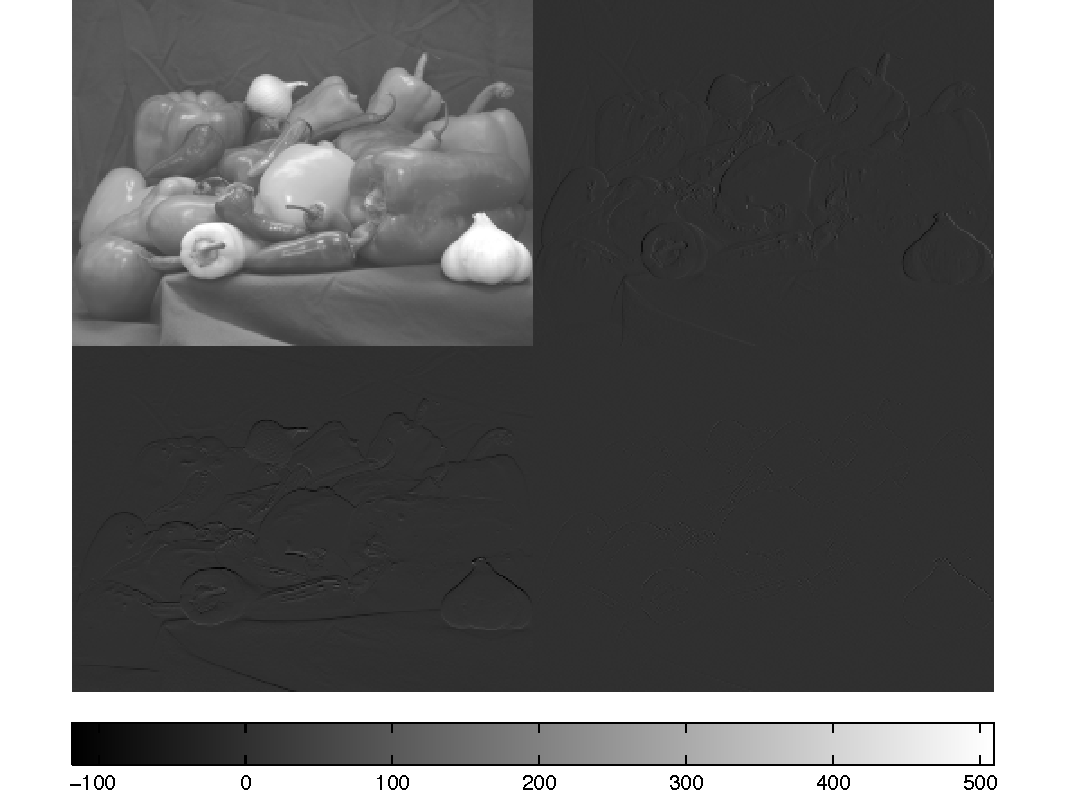
\includegraphics[width=2.5in]{../figures/haarTrans2} \quad
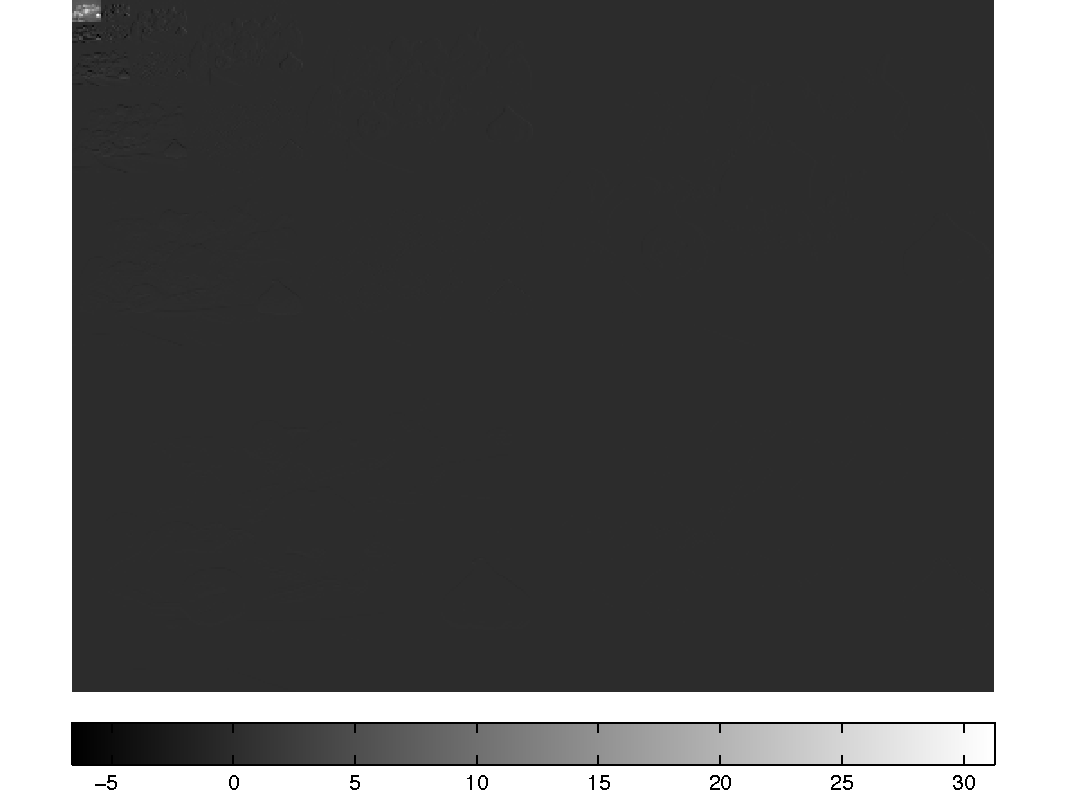
\includegraphics[width=2.5in]{../figures/haarTrans3}
\caption{a;lskdfj}
\end{figure}


WRITE MORE WRITE MORE!

Our approach considers a more general problem
\begin{equation} \label{wavelet}
\min_{x} f(Ax - b ) + \lambda \norm{Wx}_1,
\end{equation}
where $f: \R^{m \times n} \rightarrow [0,\infty)$ is some Lipschitz differentiable functional which gives a measurement of the size of the fidelity term. We specifically work with the cases 
\begin{equation} \label{fidelities}
f(x) = \begin{cases}
\norm{x}_F^2 \\
h_\gamma(x) \\
g_\gamma(x),
\end{cases}
\end{equation}
where $h_\gamma$ and $g_\gamma$ are as in \eqref{huber} and \eqref{log_cosh} respectively. 

% TV Regularization
\subsection{Total Variation Regularization}
The usual Total-Variation deblurring model, as seen in \cite{TV} can be formulated in the form of \eqref{general} as 
\begin{equation} \label{tv_orig}
\min_{x} \norm{ Ax - b }_F^2 + 2 \lambda \mathrm{TV}(x)+ \delta(x | [0,1]),
\end{equation}
where $\norm{\cdot}$ is taken as either a Frobenius norm or a 2-norm, depending on applications,  $\lambda>0$ is a regularization parameter, and $\mathrm{TV}(x)$ is the Total-Variation semi-norm.  We include the indicator function to ensure the resulting image is within the range of pixel values we are considering.  Two similar choices exist for the TV-norm: the so-called isotropic type, and the $l_1$ type.  In this work, we work exclusively with the $l_1$-based TV-norm, defined as 
$$ TV_{l_1}(x) = \sum_{i=1}^{m-1} \sum_{j=1}^{n-1} \left( \abs{x_{i,j}  - x_{i+1,j} } + \abs{ x_{i,j} - x_{i,j+1}  } \right) + \sum_{i=1}^{m-1} \abs{ x_{i,n} - x_{i+1,n} } + \sum_{j=1}^{n-1} \abs{ x_{m,j} - x_{m,j+1 } },$$
 for $x \in \R^{m \times n},$ and where the reflexive boundary conditions
\begin{align*}
x_{m+1,j} - x_{m,j} &= 0, \textrm{ for all }j \\
 x_{i,n+1} - x_{i,n} &= 0, \textrm{ for all }i
\end{align*}
are assumed.  However, it is a very simple adjustment to use the isotropic definition of total variation and all of the same methods still apply. Our approach considers a more general problem
\begin{equation} \label{tv_ours}
\min_{x} f(Ax - b ) + \lambda \mathrm{TV}_{l_1}(x) + \delta(x | [0,1]),
\end{equation}
where $f: \R^{m \times n} \rightarrow [0,\infty)$ is any functional with Lipschitz continuous gradient which gives a measurement of the size of the fidelity term.  The specific fidelity terms which we worked with were as listed in \eqref{fidelities}.

Optimization of the objective function was based on the proximal gradient algorithm and expoited the idea of momentum used in FISTA as well as an extra function evaluation at each iteration in order to ensure a non-increasing objective function.  The proximal gradient step is given as follows,

\begin{align*}
x^{k+1} &= \prox_{\alpha^{-1}(\lambda \textrm{TV}(\cdot) + \delta_{[0,1]})} (\underbrace{x^k - \alpha^{-1} A^T\nabla f (Ax^k - b)}_{u^k}) \\
&= \AMz \left( \|u^k - z\|_F^2 + \alpha^{-1}\lambda TV(z) + \delta(z | [0,1]) \right) \\
&= P_{[0,1]}  \left( \AMz \left( \|u^k - z\|_F^2 + \alpha^{-1}\lambda TV(z) \right) \right)
\end{align*}

Here the learning rate $\alpha$ is taken to be no larger than than the multiplicative inverse of the Lipschitz constant of $\nabla f$.  Note that in order to evaluate this expression we must solve a denoising problem with input $u^k = x^k - \alpha^{-1} A^T\nabla f (Ax^k - b)$.  Of particular note is that regardless of the original fidelity term we have a Frobenius norm fidelity term on the new denoising problem.  This allows for the easy manipulation of the original fidelity function, so long as it is convex and has Lipschitz gradient.

The resulting denoising problem with Frobenius norm fidelity function may be solved rapidly using the method developed in \cite{TV}.  The $TV$ function is shown to have a dual representation as a trace and the relationship between trace and Frobenius norm is heavily exploited to develop a dual formulation of the denoising problem.  We present their method here, starting with a few new definitions which will be necessary.
\begin{align*}
\mathcal{P} &= \{ (p,q) \in \R^{(m-1) \times n} \times \R^{ m \times (n-1) } :  \abs{p_{i,j} } \le 1, \abs{p_{ i,j } } \le 1 \} \\
 \mathcal{L} : \R^{(m-1) \times n} \times& \R^{ m \times (n-1) } \rightarrow \R^{m \times n}  \text{ such that } \mathcal{L}(p,q)_{i,j} = p_{i,j} + q_{i,j} - p_{ i-1,j } - q_{ i,j-1 }\\ &\hspace{3 cm} \text{ for } i = 1,\dots,m,\,j = 1,\dots,n \text{ \& }  p_{0,j} = p_{m,j} = q_{i,0} = q_{i,n} = 0\\
\end{align*}
Using these new definitions we claim without proof that the total variation functional may be written as,
\begin{equation}
TV(x) = \underset{(p,q) \in \mathcal{P}}{\max} \Tr(\mathcal{L}(p,q)^Tx)
\end{equation}
we may now exploit the relationship between trace and Frobenius norm to obtain the dual problem for Frobenius denoising using total variation regularizartion.  
\begin{align*}
\min_{x \in [0,1]} \norm{x-b}_F^2 +2 \lambda \mathrm{TV}(x) &= \min_{x \in [0,1]}  \underset{(p,q) \in \mathcal{P}}{\max}  \norm{x-b}_F^2 + 2\lambda \Tr(\mathcal{L}(p,q)^Tx) \\
&= \underset{(p,q) \in \mathcal{P}}{\max}   \min_{x \in [0,1]} \norm{x-b}_F^2 +2 \lambda \Tr(\mathcal{L}(p,q)^Tx) \\
&=\underset{(p,q) \in \mathcal{P}}{\max}   \min_{x \in [0,1]} \norm{x}_F^2 + \norm{b}_F^2 - 2 \Tr(x^Tb)+ 2\lambda \Tr(\mathcal{L}(p,q)^Tx) \\
&=\underset{(p,q) \in \mathcal{P}}{\max}   \min_{x \in [0,1]} \norm{x}_F^2 + \norm{b}_F^2 - 2 \Tr(x^T(b- \lambda\mathcal{L}(p,q)))\\
&=\underset{(p,q) \in \mathcal{P}}{\max}   \min_{x \in [0,1]} \underbrace{\norm{x}_F^2 + \norm{b- \lambda\mathcal{L}(p,q)}_F^2 - 2 \Tr(x^T(b- \lambda\mathcal{L}(p,q)))}_{ = \norm{x-(b- \lambda\mathcal{L}(p,q))}_F^2} -  \norm{b- \lambda\mathcal{L}(p,q)}_F^2+ \norm{b}_F^2\\
&= \underset{(p,q) \in \mathcal{P}}{\max}   \min_{x \in [0,1]}  \norm{x-(b- \lambda\mathcal{L}(p,q))}_F^2 - \norm{b- \lambda\mathcal{L}(p,q)}_F^2+ \norm{b}_F^2
\end{align*}
Here the switching of min and max is permitted due to the convexity of the objective in $x$ and concavity in $p$ and $q$ \cite{TV}.  Note that the problem of maximizing over $x$ is simply the projection of each index of  $b- \lambda\mathcal{L}(p,q)$ onto the set $[0,1]$.  This gives the optimality condition for $x$ in terms of $p$ and $q$ which we plug back in to obtain the dual problem.
\begin{align*}
(p^*,q^*) &= \underset{(p,q) \in \mathcal{P}}{\text{arg }\max}  \norm{P_{[0,1]}(b- \lambda\mathcal{L}(p,q)) -(b- \lambda\mathcal{L}(p,q))}_F^2 - \norm{b- \lambda\mathcal{L}(p,q)}_F^2+ \norm{b}_F^2\\
x &= P_{[0,1]}(b- \lambda\mathcal{L}(p^*,q^*))
\end{align*}
Note that in the dual problem the objective is Lipschitz differentiable.  We claim without proof that the gradient has Lipschitz constant $L \leq 16 \lambda^2$ and refer the reader to \cite{TV} for proof.  This smoothness allows us to implement a projected gradient algorithm which we discuss in the next section.

% Algorithms
\section{Algorithms}
A simple way to solve for the real image $x$ give $g(x) = 0$ is to apply the gradient descent algorithm,

\begin{equation}
x_k = x_{k-1} - t_k \nabla f(x_{k-1}),
\end{equation}

for suitable stepsize $t_k > 0$. When $g$ is nontrivial and nonsmooth (the usual case), we can rewrite this as a proximal mapping,

\begin{equation}
\prox_g(x_{k-1} - \nabla f(x_{k-1})) = \min_x \left( \frac{1}{2}||x-x_{k-1} - \nabla f(x_{k-1})||_2^2  + \lambda g(x)\right)
\end{equation}

The advantage of this form is that many nonsmooth regularizers have a close formed solution for their $\prox$.


\begin{minipage}{0.48\textwidth}
\textbf{MFISTA$(b,f, \lambda)$}
\begin{algorithmic}
\State $y^1 = x^0 = b; \, t^1 = 1$
\State $\alpha \geq Lip(\nabla f)$
\For {$k = 1:N$}
	\State $u^k = y^k - \frac{A^T\nabla f (A y^k - b)}{\alpha}$
	\State $z^k = FGP(u^k, \frac{\lambda}{2 \alpha})$
	\State $x^k = \underset{x \in \{x^{k-1},z^k\}}{\text{argmin}} \,L_b(x)$
	\State $t^{k+1} = \frac{1 + \sqrt{1 + 4{t^k}^2}}{2}$ 
	\State $y^{k+1} = x^k + \frac{t^k}{t^{k+1}}(z^k - x^k)$ 
	\State \hspace{10 mm}$+ \frac{t^{k-1}}{t^{k+1}}(z^k - x^k) $
\EndFor\\
\Return $x^N$
\end{algorithmic}
\end{minipage}
\begin{minipage}{0.48\textwidth}

\textbf{FGP$(b, \lambda)$}
\begin{algorithmic}
\State $(r_{ij}^1, s_{ij}^1) = (p_{ij}^0, q_{ij}^0) = 0; \, t^1 = 1$
\For {$k = 1:N$}
	\State $(p^k,q^k) = P_\mathcal{P} \left( (r^k,s^k) - \frac{\mathcal{L}^TP_{[0,1]} (b - \lambda \mathcal{L}(r^k,s^k))}{8\lambda} \right)$
	\State $t^{k+1} = \frac{1 + \sqrt{1 + 4{t^k}^2}}{2}$ 
	\State $(r^k,s^k) = (p^k,q^k) + \frac{t^k-1}{t^{k+1}}(p^k-p^{k-1}, q^k-q^{k-1})$ 
\EndFor \\
\Return $P_{[0,1]} (b - \lambda \mathcal{L}(p^N,q^N))$
\end{algorithmic}

\end{minipage}

\subsection{Wavelet Regularization}

\subsection{Total Variation Regularization}

% Examples
\section{Examples}

\subsection{Wavelet Regularization}


\begin{figure}[H]
\begin{center}
\rotatebox{90}{\hspace{1cm} Original Image \hspace{3cm} Frobenius Loss}
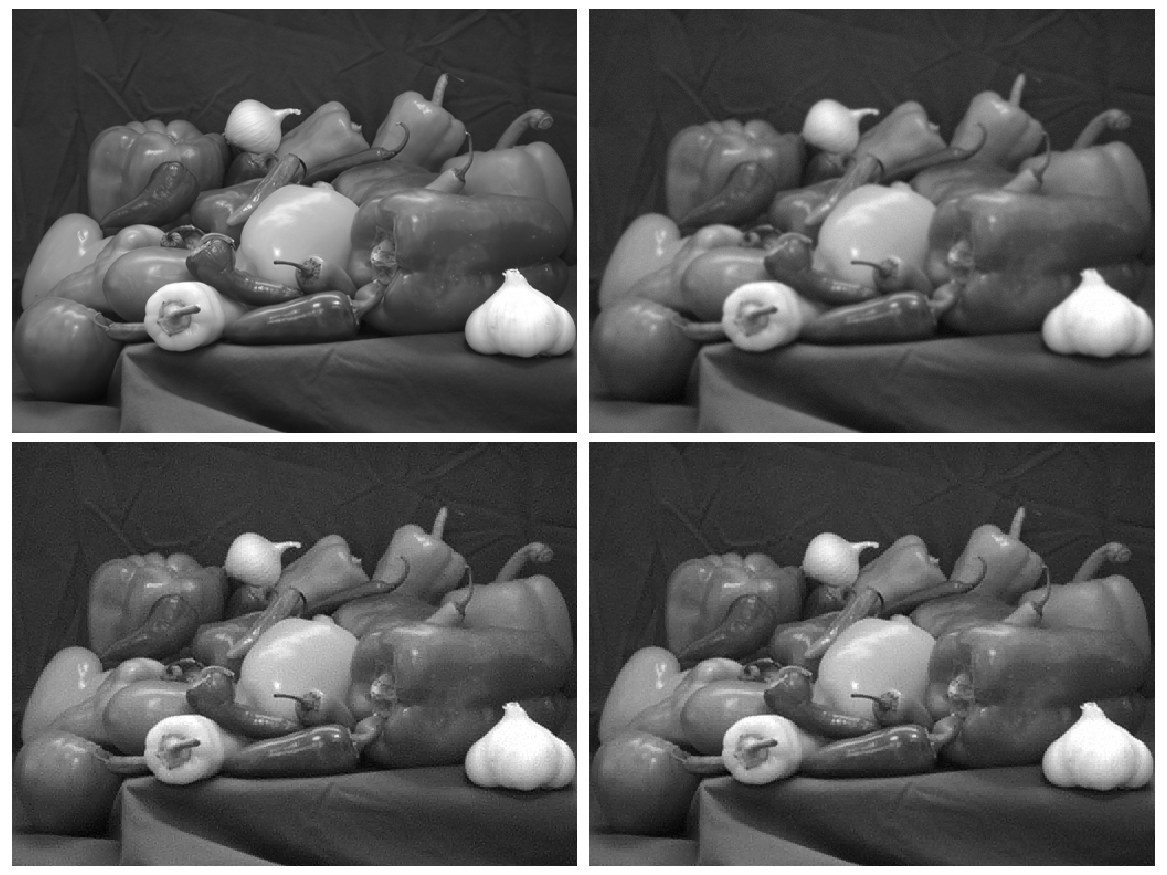
\includegraphics[width = 0.75\textwidth]{../figures/waveletGaussH.pdf} 
\rotatebox{270}{\hspace{-9cm} Blurred and Noisy \hspace{2.6cm} Huber Loss}
\end{center}
\caption{$\ell_1$ Wavelet algorithm performed on an image with Gaussian noise (magnitude $1 \times 10^{-3}$) for the two different fidelity terms of Frobenius and Huber loss. This method used the Haar wavelet for deblurring.}
\label{waveletH_gauss}
\end{figure}

\begin{figure}[H]
\begin{center}
\rotatebox{90}{\hspace{1cm} Original Image \hspace{3cm} Frobenius Loss}
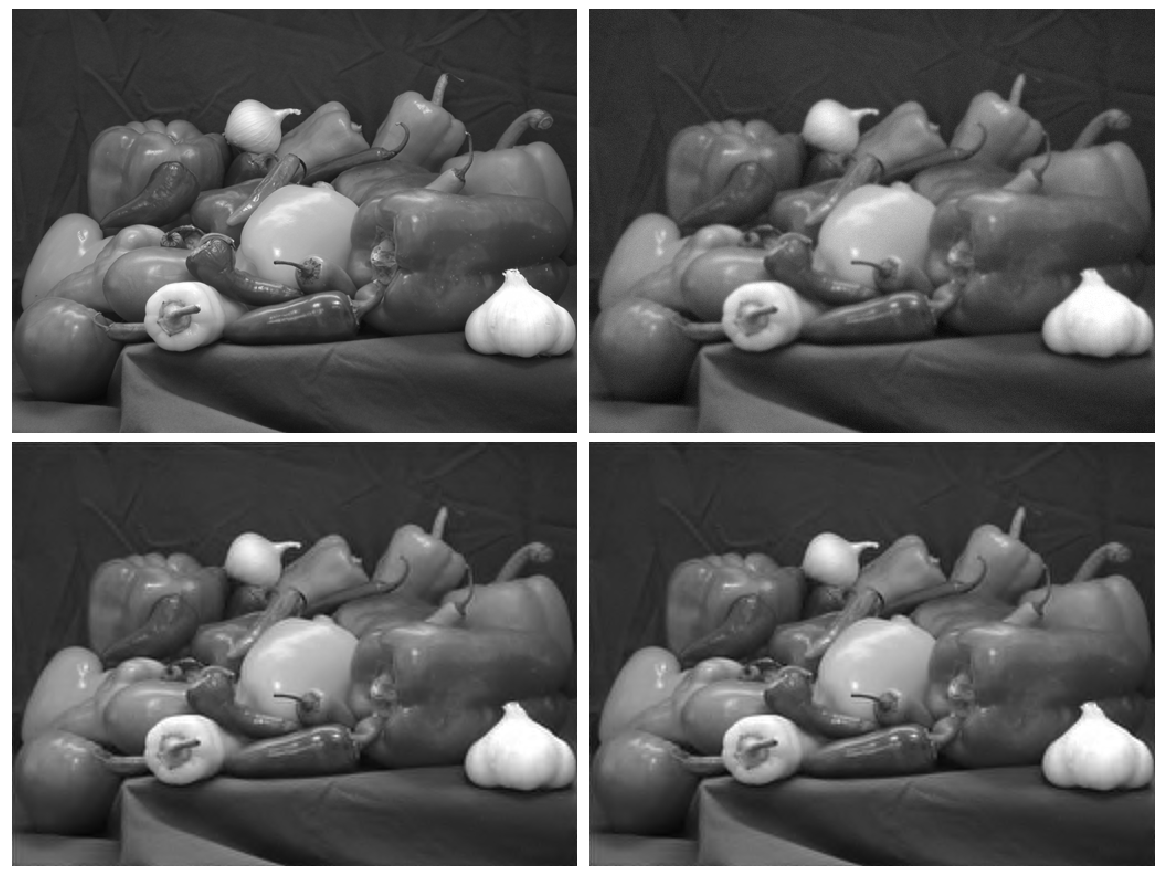
\includegraphics[width = 0.75\textwidth]{../figures/waveletGaussD.pdf} 
\rotatebox{270}{\hspace{-9cm} Blurred and Noisy \hspace{2.6cm} Huber Loss}
\end{center}
\caption{$\ell_1$ Wavelet algorithm performed on an image with Gaussian noise (magnitude $1 \times 10^{-3}$) for the two different fidelity terms of Frobenius and Huber loss. This method used the Daubechies wavelet for deblurring.}
\label{waveletD_gauss}
\end{figure}

\begin{figure}[H]
\begin{center}
\rotatebox{90}{\hspace{1cm} Original Image \hspace{3cm} Frobenius Loss}
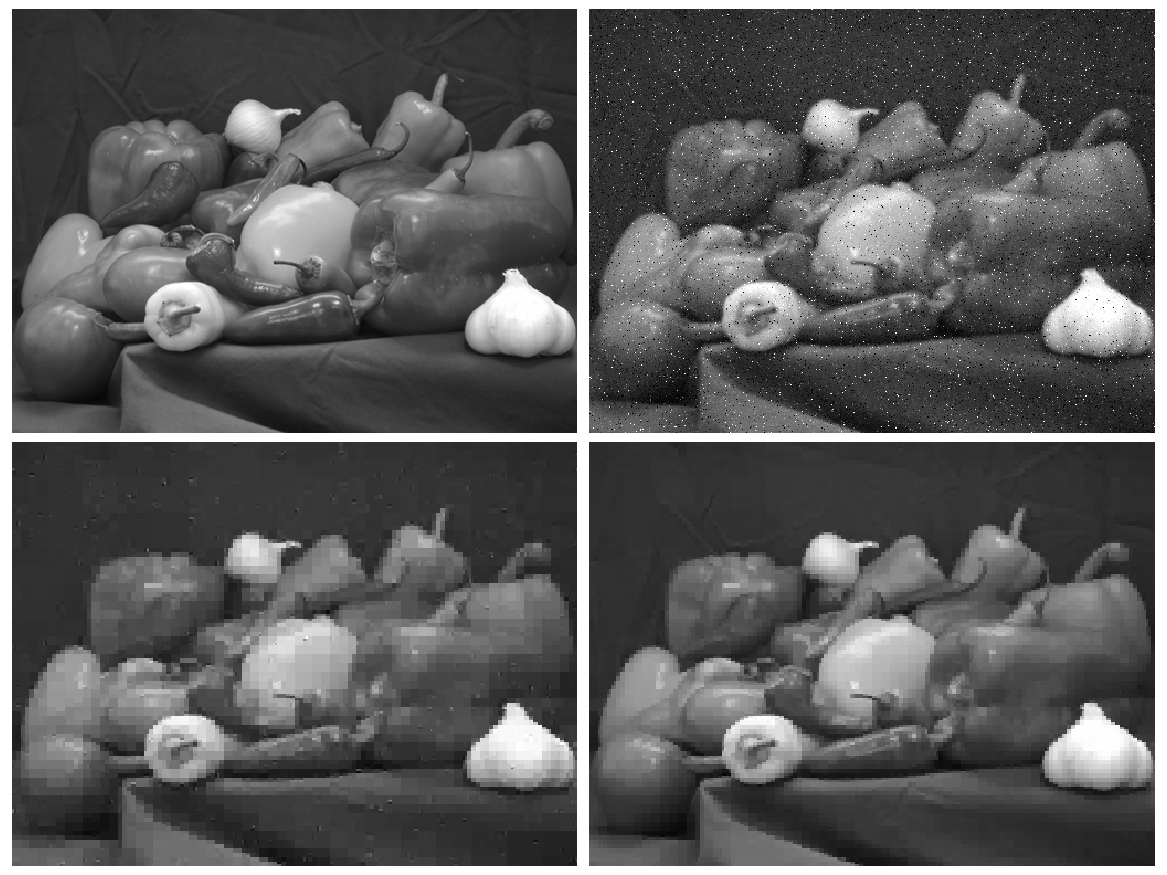
\includegraphics[width = 0.75\textwidth]{../figures/waveletStudentH.pdf} 
\rotatebox{270}{\hspace{-9cm} Blurred and Noisy \hspace{2.6cm} Huber Loss}
\end{center}
\caption{$\ell_1$ Wavelet algorithm performed on an image with Student's t noise (magnitude $1 \times 10^{-4}$) for the two different fidelity terms of Frobenius and Huber loss. This method used the Haar wavelet for deblurring.}
\label{waveletH_student}
\end{figure}

\begin{figure}[H]
\begin{center}
\rotatebox{90}{\hspace{1cm} Original Image \hspace{3cm} Frobenius Loss}
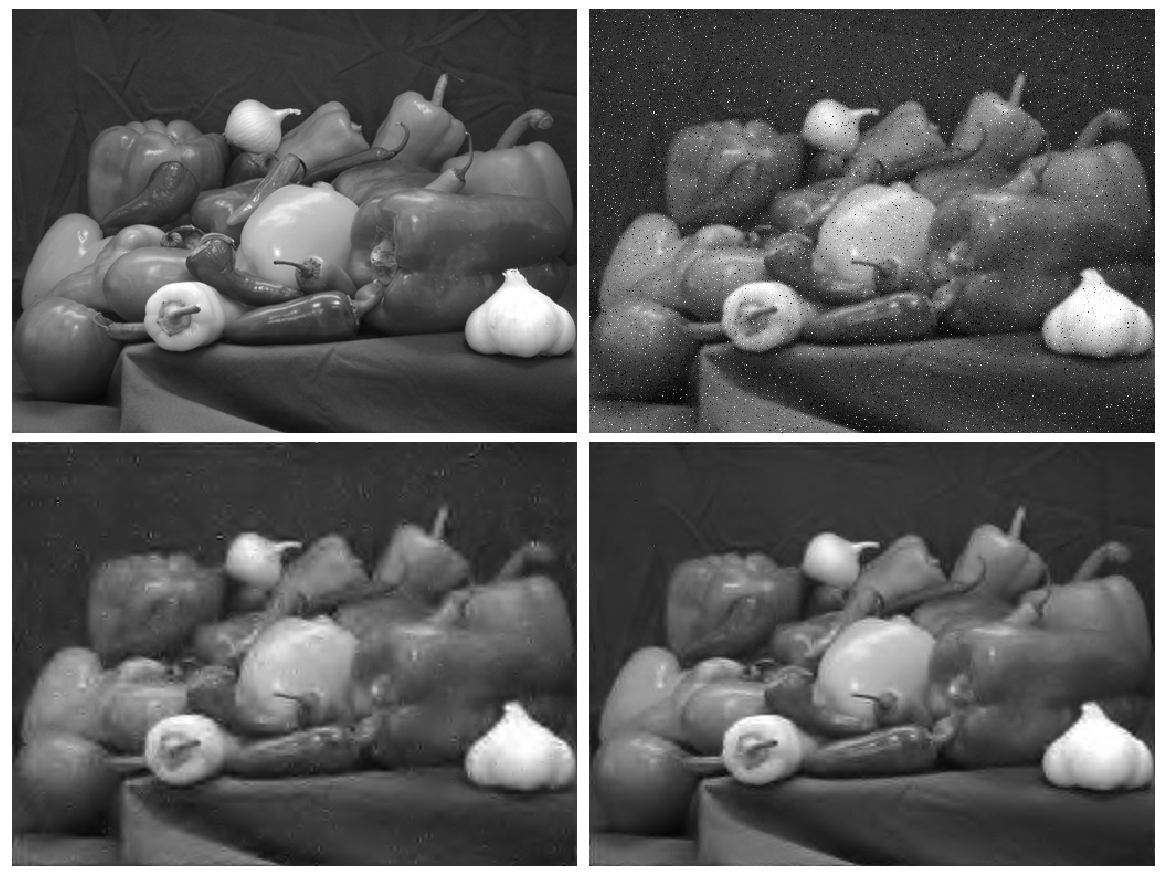
\includegraphics[width = 0.75\textwidth]{../figures/waveletStudentD.pdf} 
\rotatebox{270}{\hspace{-9cm} Blurred and Noisy \hspace{2.6cm} Huber Loss}
\end{center}
\caption{$\ell_1$ Wavelet algorithm performed on an image with Student's t noise (magnitude $1 \times 10^{-4}$) for the two different fidelity terms of Frobenius and Huber loss. This method used the Daubechies wavelet for deblurring.}
\label{waveletD_student}
\end{figure}

\subsection{Total Variation Regularization}

We demonstrate some results of denoising and deblurring with the Total Variation regularization on real images. As previously shown, each image was given a small amount of either Gaussian or Student's t noise and blurred. Two different fidelity functions were used: the squared Frobenius norm, and the Huber norm. Figure \ref{tv_gauss} demonstrates the results using Gaussian noise, and Figure \ref{tv_student} demonstrates the results using Student's t noise with one degree of freedom. For the Gaussian noise, we set $\lambda = .001$, and $\gamma = .02$ (see TV-regularization in Problem Formulation). For Student's t noise, we set $\lambda = .002$, and $\gamma = .02$.

\begin{figure}[H]
\begin{center}
\rotatebox{90}{\hspace{1cm} Original Image \hspace{3cm} Frobenius Loss}
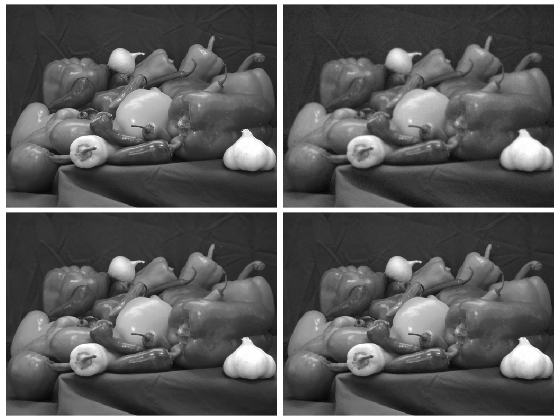
\includegraphics[width = 0.75\textwidth]{../figures/gaussian_peppers.png} 
\rotatebox{270}{\hspace{-9cm} Blurred and Noisy \hspace{2.6cm} Huber Loss}
\end{center}
\caption{Total Variation algorithm performed on an image with Gaussian noise (magnitude $1 \times 10^{-3}$) for the two different fidelity terms of Frobenius and Huber loss.}
\label{tv_gauss}
\end{figure}

\begin{figure}[H]
\begin{center}
\rotatebox{90}{\hspace{1cm} Original Image \hspace{3cm} Frobenius Loss}
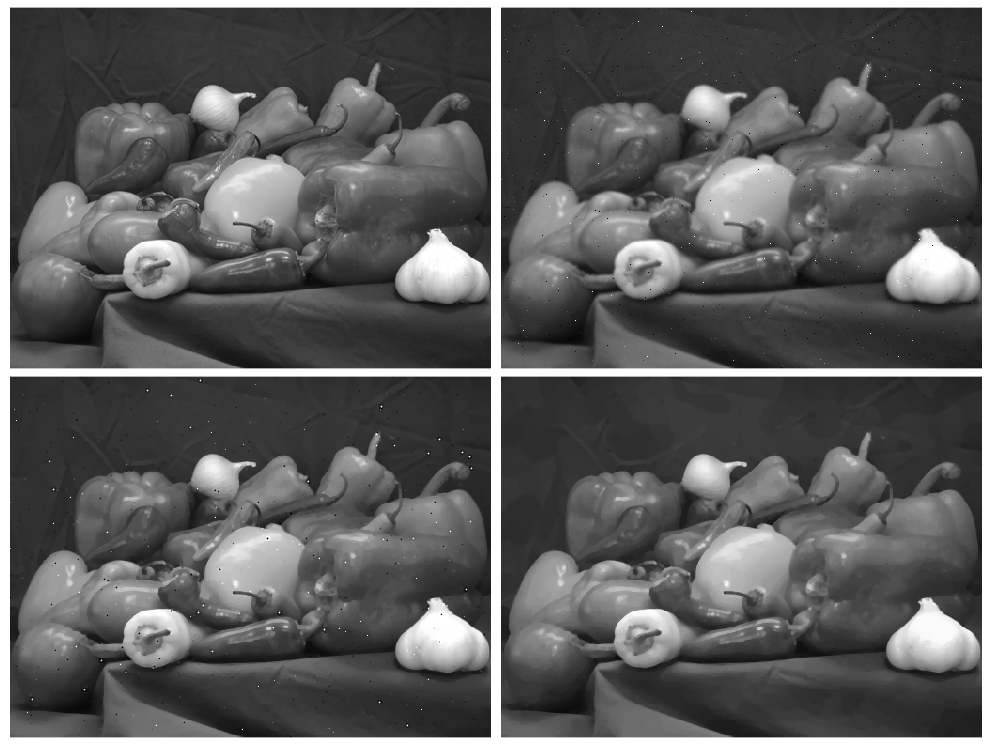
\includegraphics[width = 0.75\textwidth]{../figures/student-t_peppers.png} 
\rotatebox{270}{\hspace{-9cm} Blurred and Noisy \hspace{2.6cm} Huber Loss}
\end{center}
\caption{Total Variation algorithm performed on an image with Student's t noise (magnitude $1 \times 10^{-4}$) for the two different fidelity terms of Frobenius and Huber loss.}
\label{tv_student}
\end{figure}

\subsection{The $\log \circ \cosh$ Penalty Function}

Recall that for large values of $\gamma$ the function $\gamma^{-1} \log(\cosh (\gamma \cdot ))$ uniformly converges to the absolute value function.  Since it is also Lipschitz differentiable we are able to use it in our algorithm for TV regularized denoising and deblurring with high values of $\gamma$ to approximate how the standard $L^1$ norm would perform without needing to worry about how to optimize it.

\begin{figure}[H]
	\begin{center}
	    \rotatebox{90}{\hspace{1cm} $\log \circ \cosh$ Loss \hspace{3cm} Original Image}
		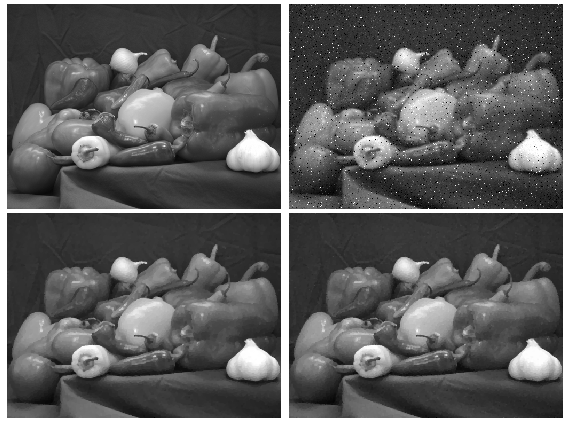
\includegraphics[width=0.8\textwidth]{../figures/logcosh_peppers.png}
		\rotatebox{270}{\hspace{-9cm} Blurred and Noisy \hspace{2.6cm} Huber Loss}
		\caption{A comparrison between the $\log \circ \cosh$ and Huber Fidelity Terms }
		\label{comp_methods}
	\end{center}
\end{figure}

To do:
-it seems to perform better
-it also takes longer since the step size decreases like 1/gamma

% Discussion
\section{Discussion and Conclusions}

\begin{figure}[H]
	
	\begin{center}
		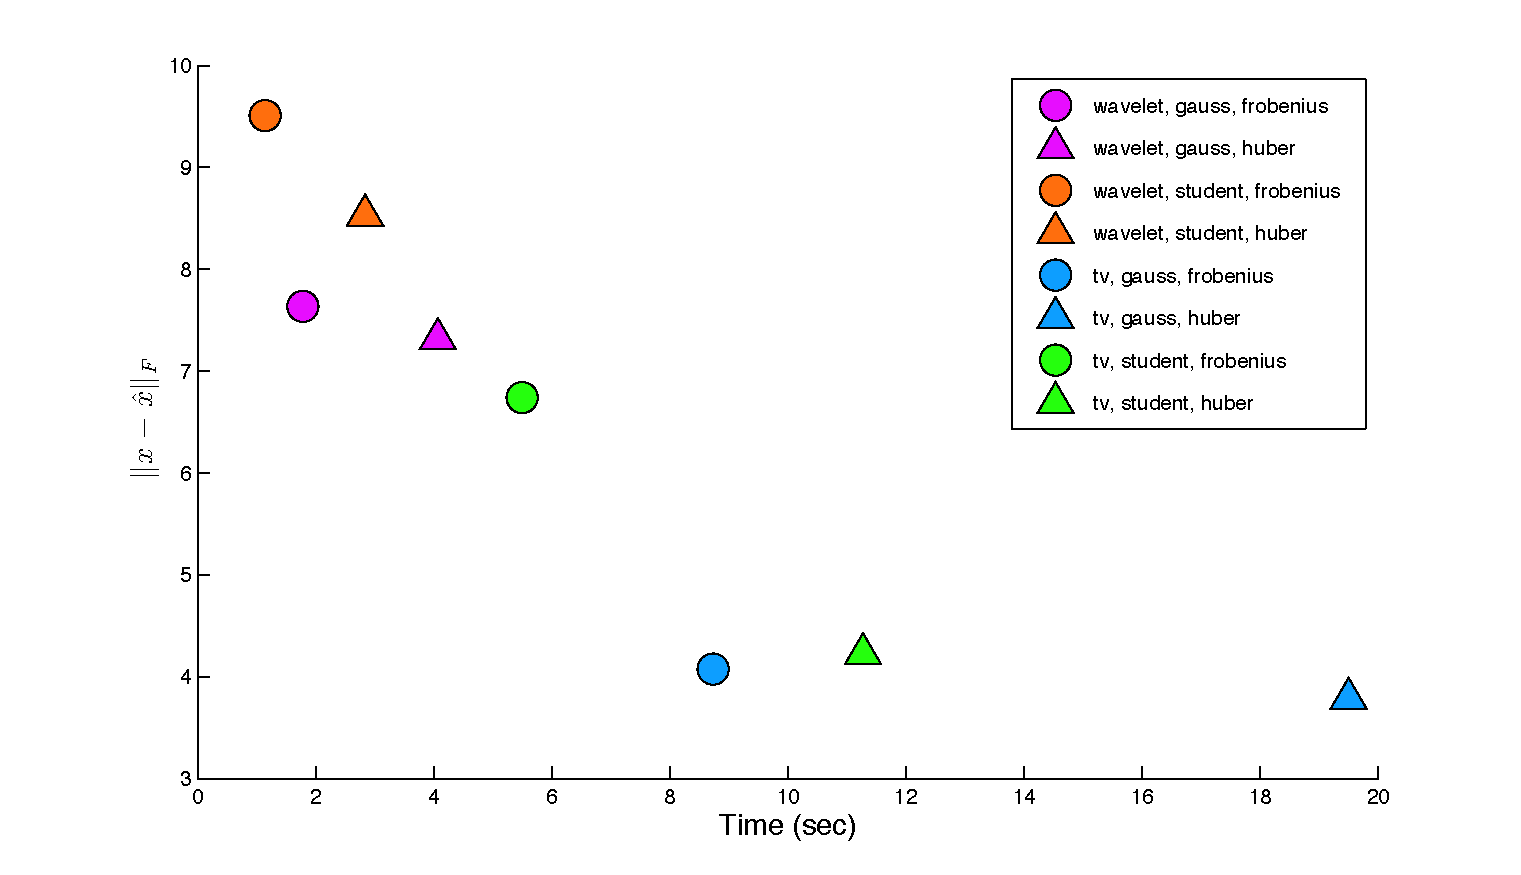
\includegraphics[width=0.8\textwidth]{../figures/comparePlot2.pdf}
		\caption{Timing information and the Frobenius norm error between the true and observed image until the relative change in the objective function is less than $.001$. }
		\label{comp_methods}
	\end{center}
\end{figure}


Figure \ref{comp_methods} shows a rough comparison of our methods by displaying the time complexity and Frobenius error for different fidelity functions, regularization techniques and noise-types. It is clear that TV regularization outperformed wavelet regularization at the price of additional computational complexity. This is not surprising due to TV's extra requirement of solving an inner optimization problem for denoising the image. It can also be seen that student noise generally required less time than Gaussian noise but at the expense of higher error. Finally, applying the Huber for student noise improved results drastically for a slight increase in computation time.  

In conclusion, we present a survey of regularization and fidelity functions for the image denoising/deblurring problem. In particular, we compare regularization of the 1-norm in the wavelet domain to TV regularization. Furthermore we explore the affect of using the Huber as a fidelity function and potential improvements it can have when applied to heavy tailed noise. Our results show that TV regularization performs better for high amounts of noise, but the wavelet domain is well suited for smaller amounts of noise due to computational speed improvements. 

In our research we came across many challenges and avenues for future work. It is clear from \ref{lambda_find}, that the correct choice of the regularization parameter is very important for maximizing results. However, the correct value varies for different classes of images. Therefore, there is a high need for finding the correct value for the regularization parameter across images. Additionally, finding an appropriate error metric can be a difficult challenge when quantitatively analyzing performance for the methods shown. The Frobenius norm of the error is the most common metric, but does can do a poor job of correctly evaluating the improvements from denoising and deblurring algorithms due to large structural changes of the images. 





%\printbibliography[title={Sources}]
\bibliographystyle{unsrt}
\bibliography{sources}


\end{document}